% ---------------------------- TOPOGRAPHY ---------------------------- 
\begin{table*}[h]
\small\sf\centering
\caption{Topographic experiment: maps of raster statistics and geospatial analyses draped over 3D topography for all participants.}
\ra{1.3}
\begin{tabular}{m{0.16\textwidth} m{0.18\textwidth} m{0.18\textwidth} m{0.18\textwidth} m{0.18\textwidth}}
\toprule
& \multicolumn{1}{c}{Reference} & \multicolumn{1}{c}{Digital} & \multicolumn{1}{c}{Analog}  & \multicolumn{1}{c}{Tangible}\\
\midrule
%
Mean elevation \par \vspace{0.5em} 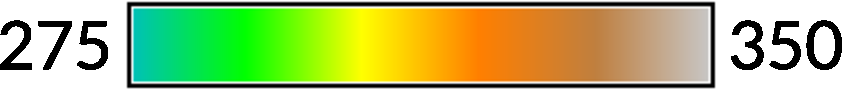
\includegraphics[width=0.16\textwidth]{images/legends/elevation_legend_1.pdf} & 
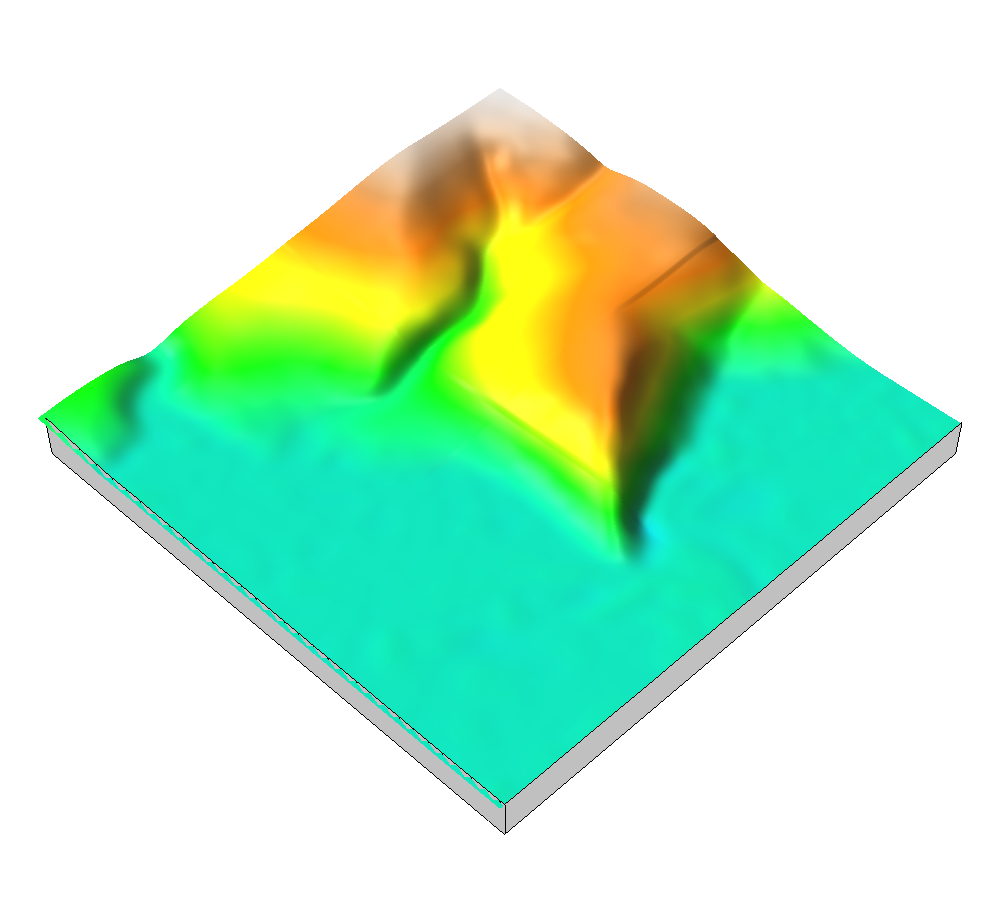
\includegraphics[width=0.18\textwidth]{images/render_3d/participants/dem_1.png} &
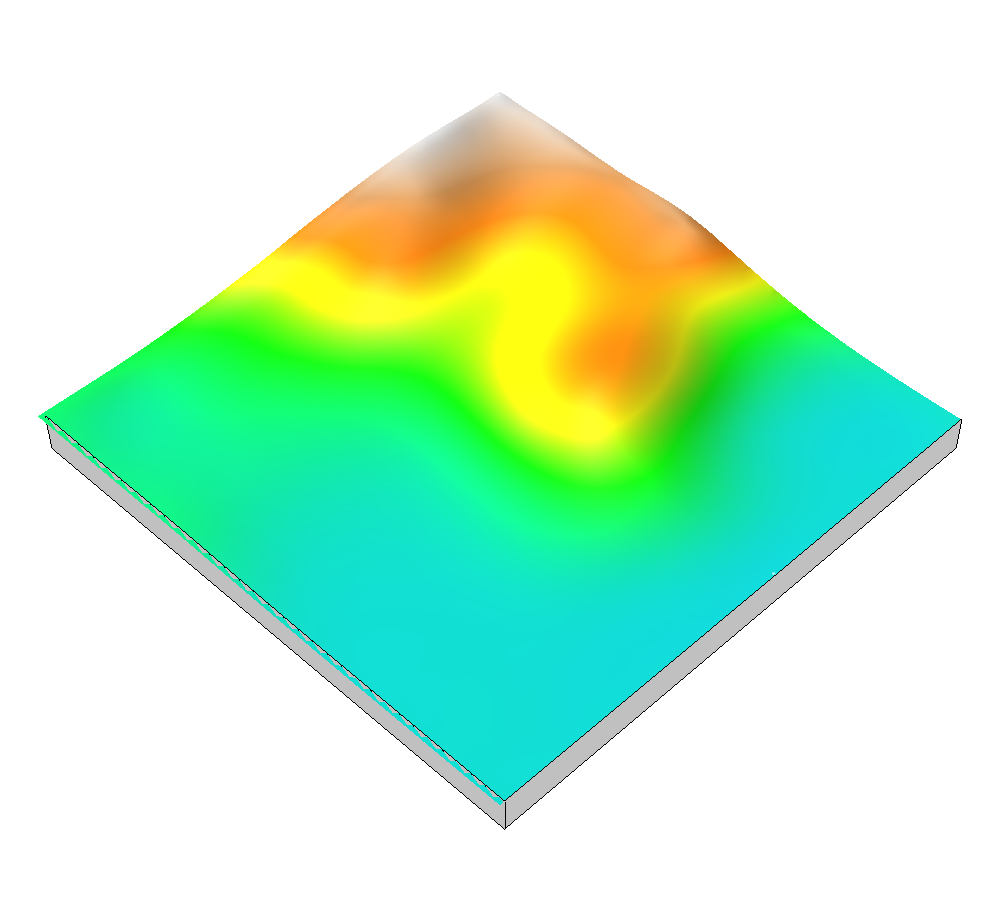
\includegraphics[width=0.18\textwidth]{images/render_3d/participants/mean_dem_1.png} &
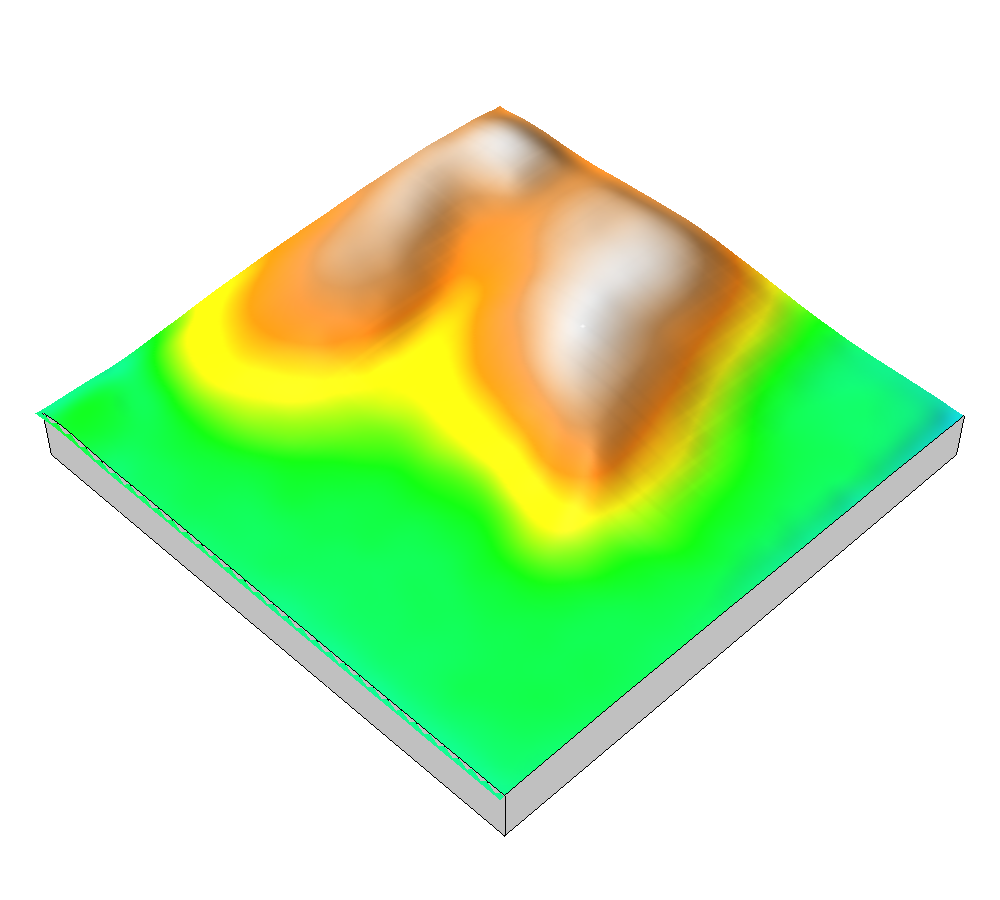
\includegraphics[width=0.18\textwidth]{images/render_3d/participants/mean_dem_2.png} &
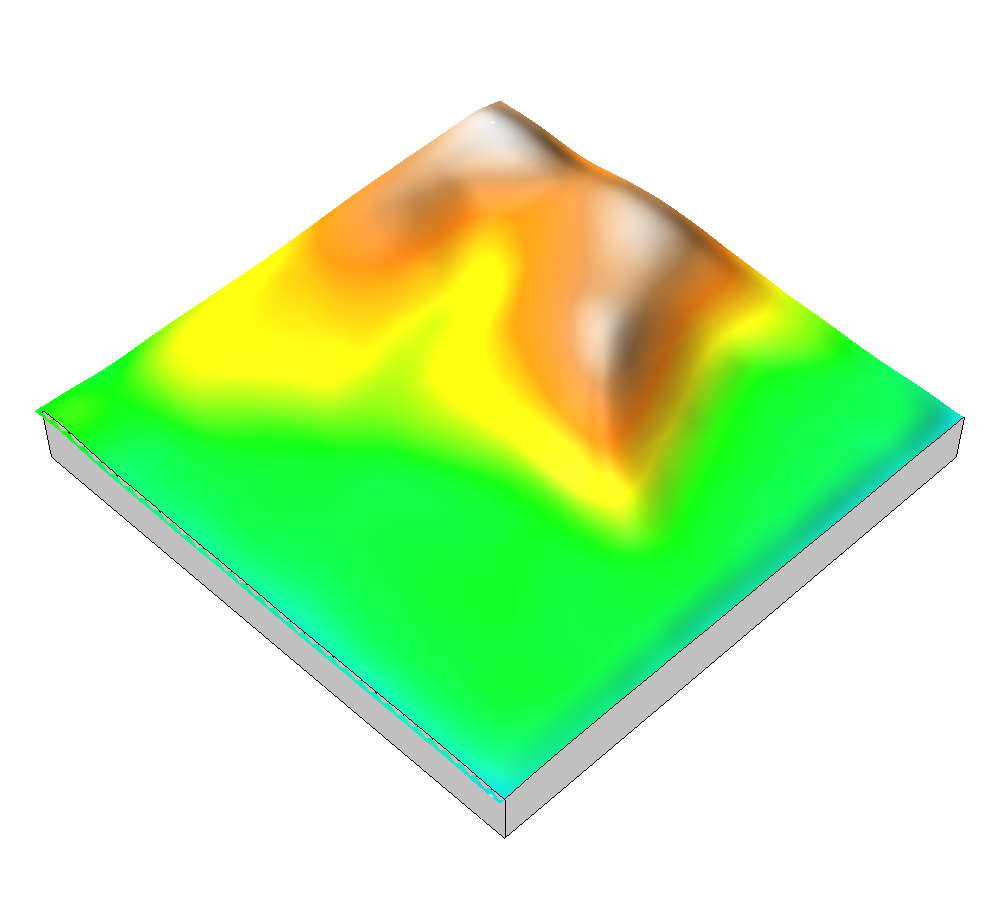
\includegraphics[width=0.18\textwidth]{images/render_3d/participants/mean_dem_3.png}\\
%
Stdev.~of elevations \par \vspace{0.5em} 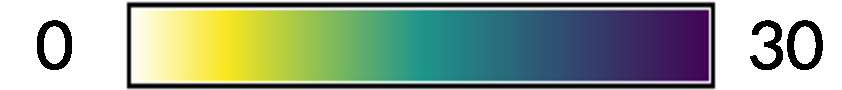
\includegraphics[width=0.16\textwidth]{images/legends/stdev_legend.pdf} & 
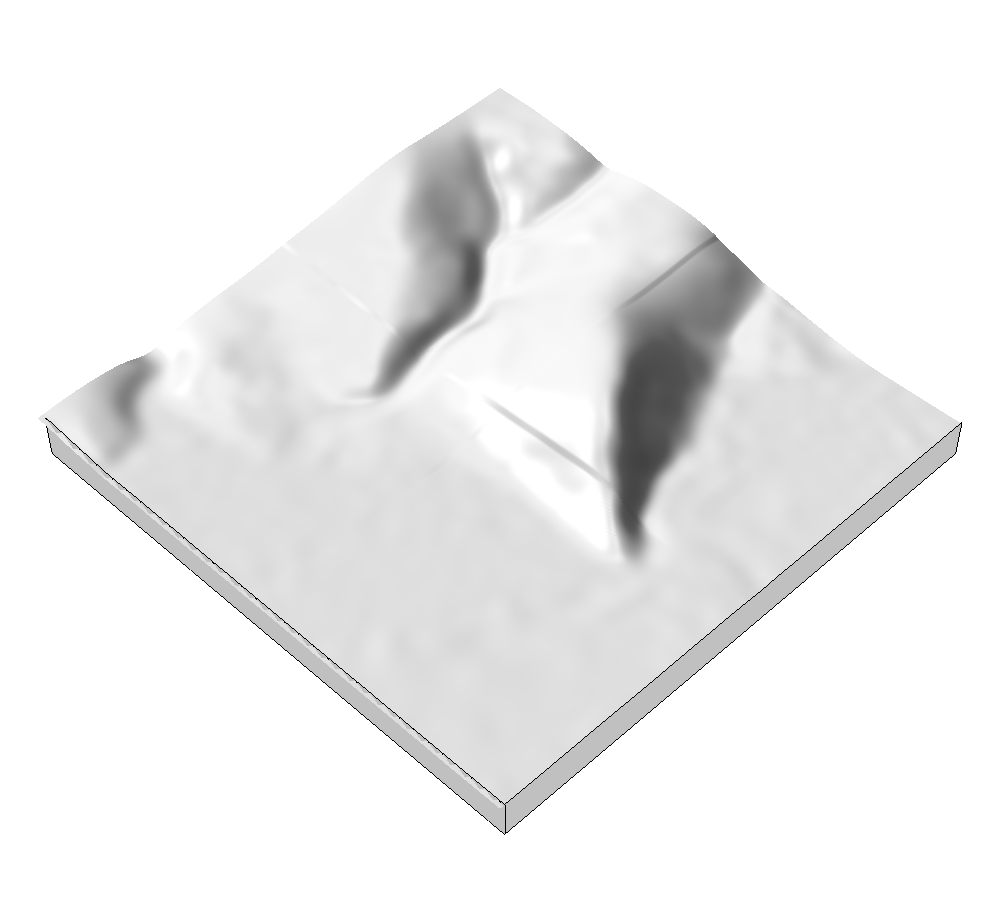
\includegraphics[width=0.18\textwidth]{images/render_3d/participants/dem_difference_1.png} &
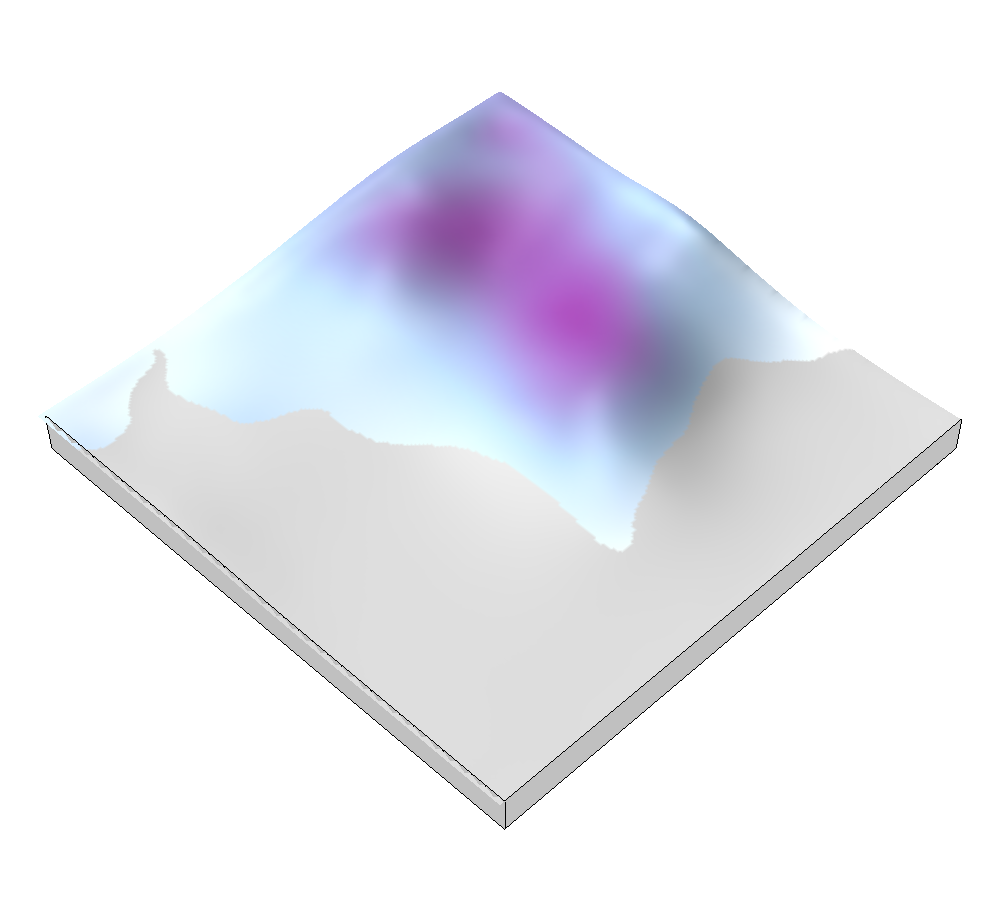
\includegraphics[width=0.18\textwidth]{images/render_3d/participants/stdev_dem_1.png} &
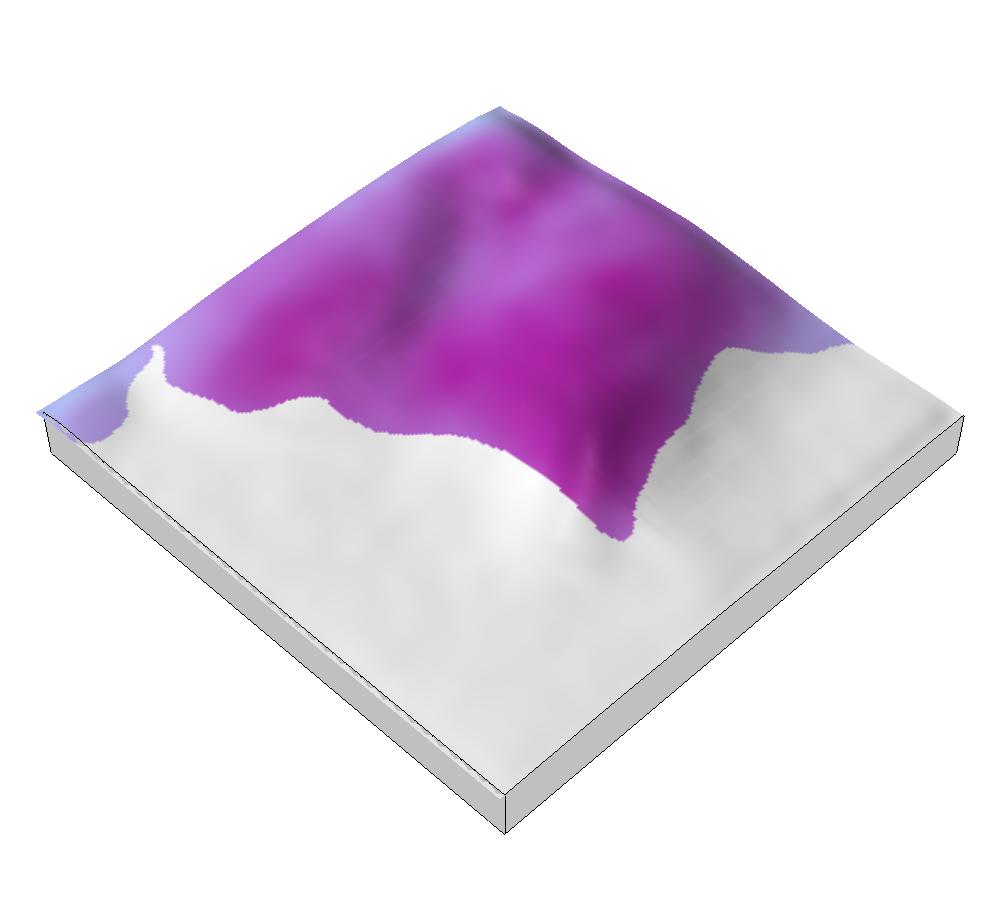
\includegraphics[width=0.18\textwidth]{images/render_3d/participants/stdev_dem_2.png} &
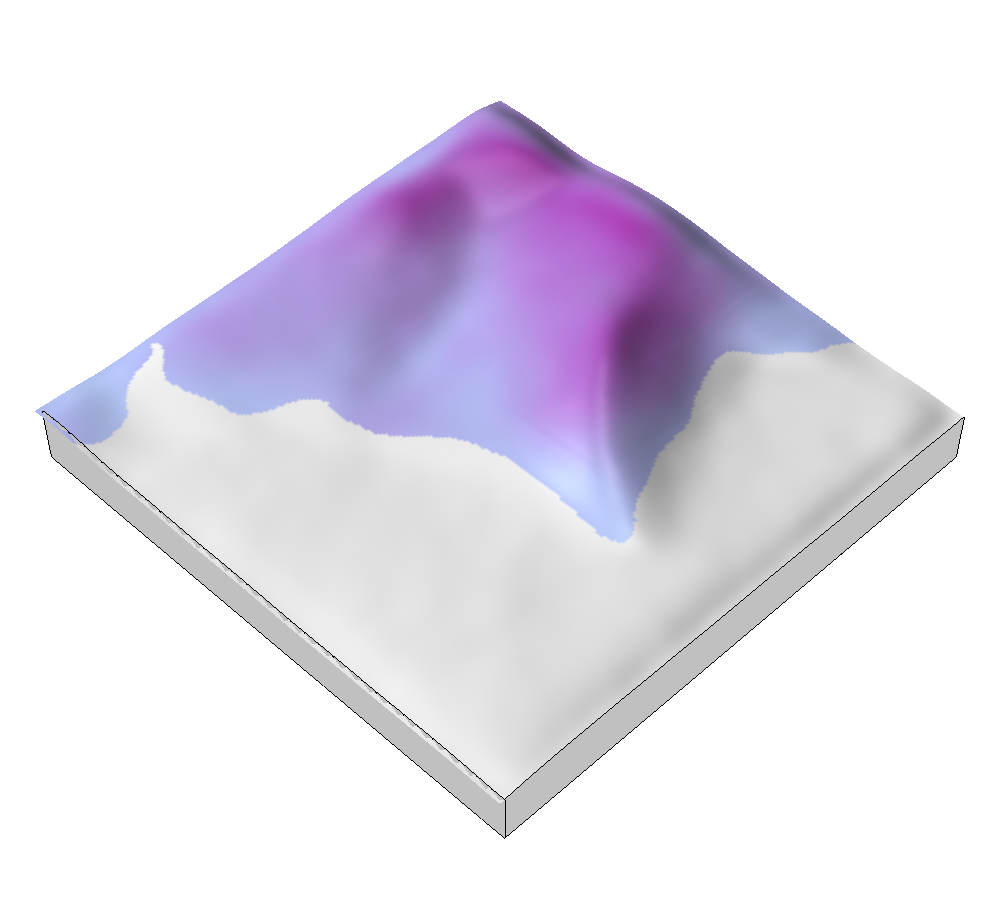
\includegraphics[width=0.18\textwidth]{images/render_3d/participants/stdev_dem_3.png}\\
%
Stdev.~of difference \par \vspace{0.5em} 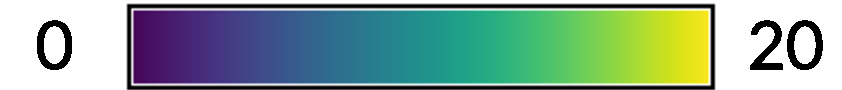
\includegraphics[width=0.16\textwidth]{images/legends/stdev_diff_legend.pdf} & 
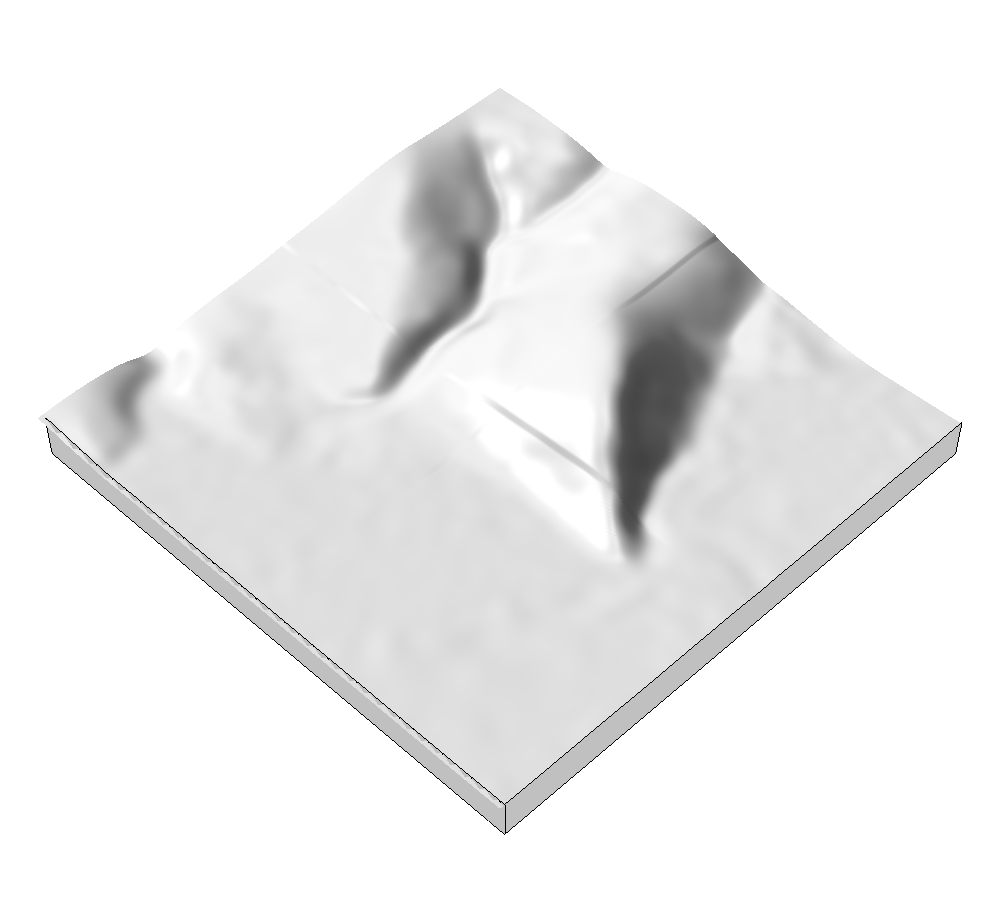
\includegraphics[width=0.18\textwidth]{images/render_3d/participants/dem_difference_1.png} &
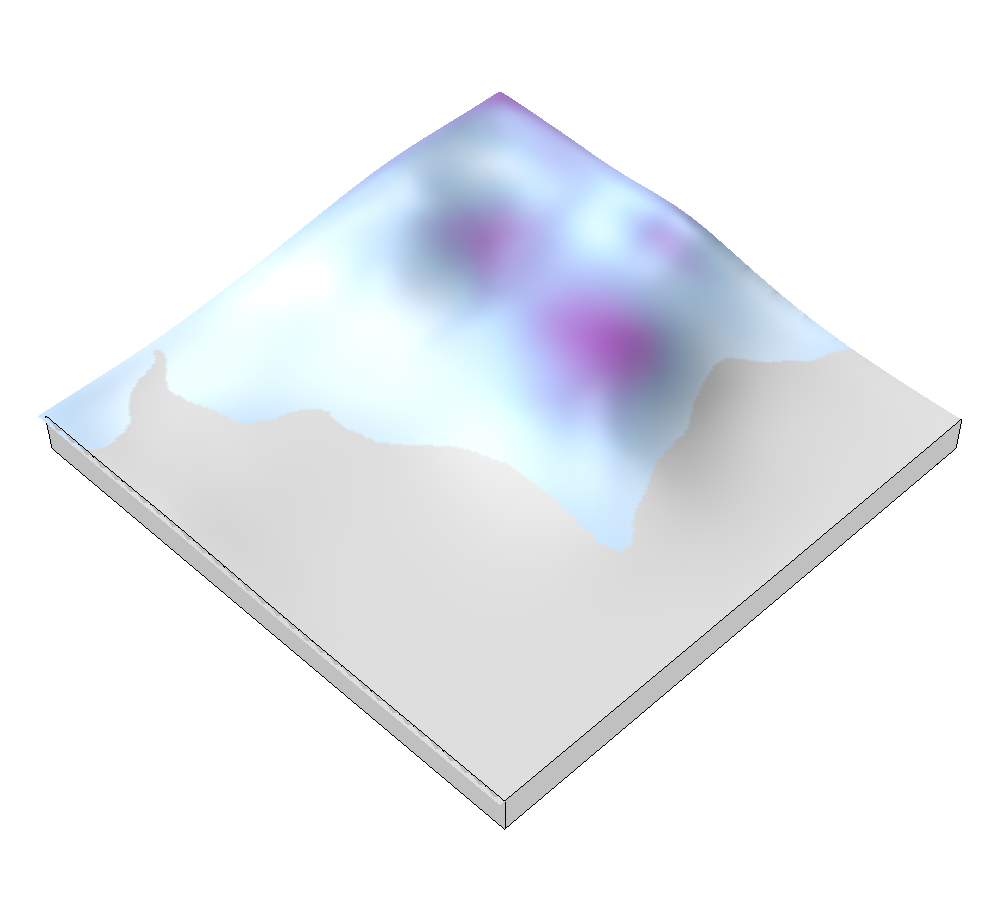
\includegraphics[width=0.18\textwidth]{images/render_3d/participants/stdev_regression_difference_series_1.png} &
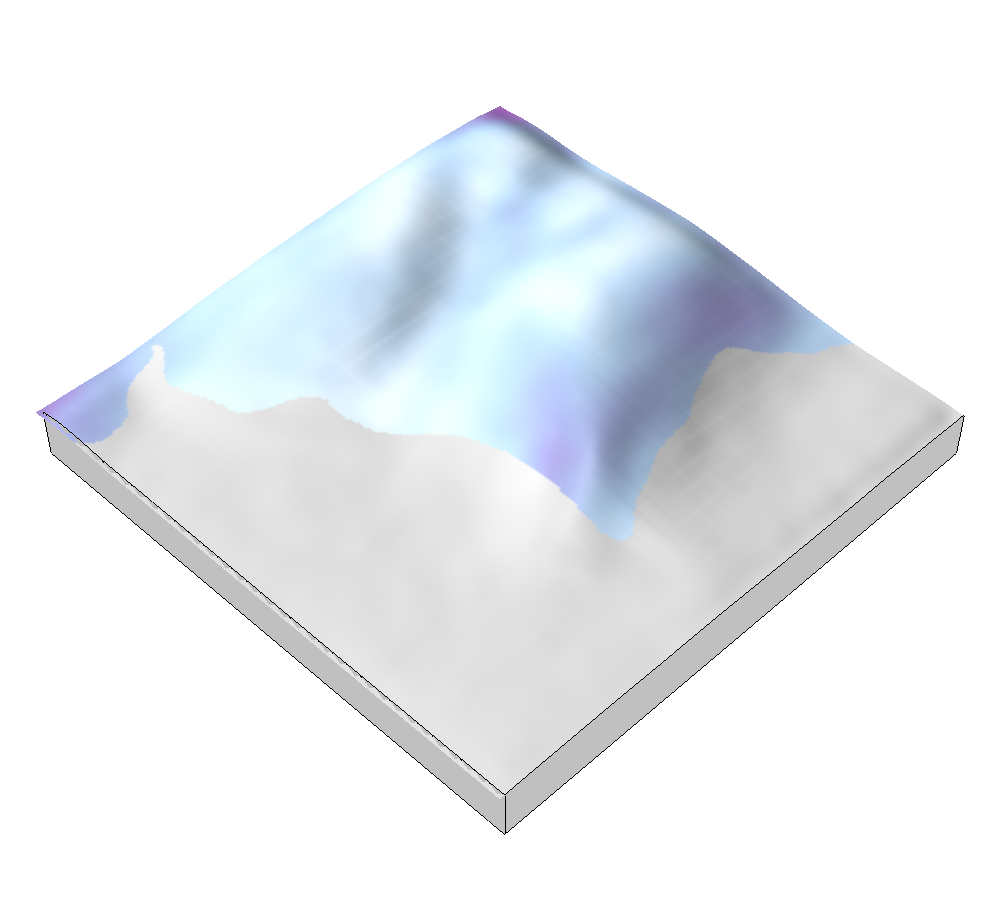
\includegraphics[width=0.18\textwidth]{images/render_3d/participants/stdev_regression_difference_series_2.png} &
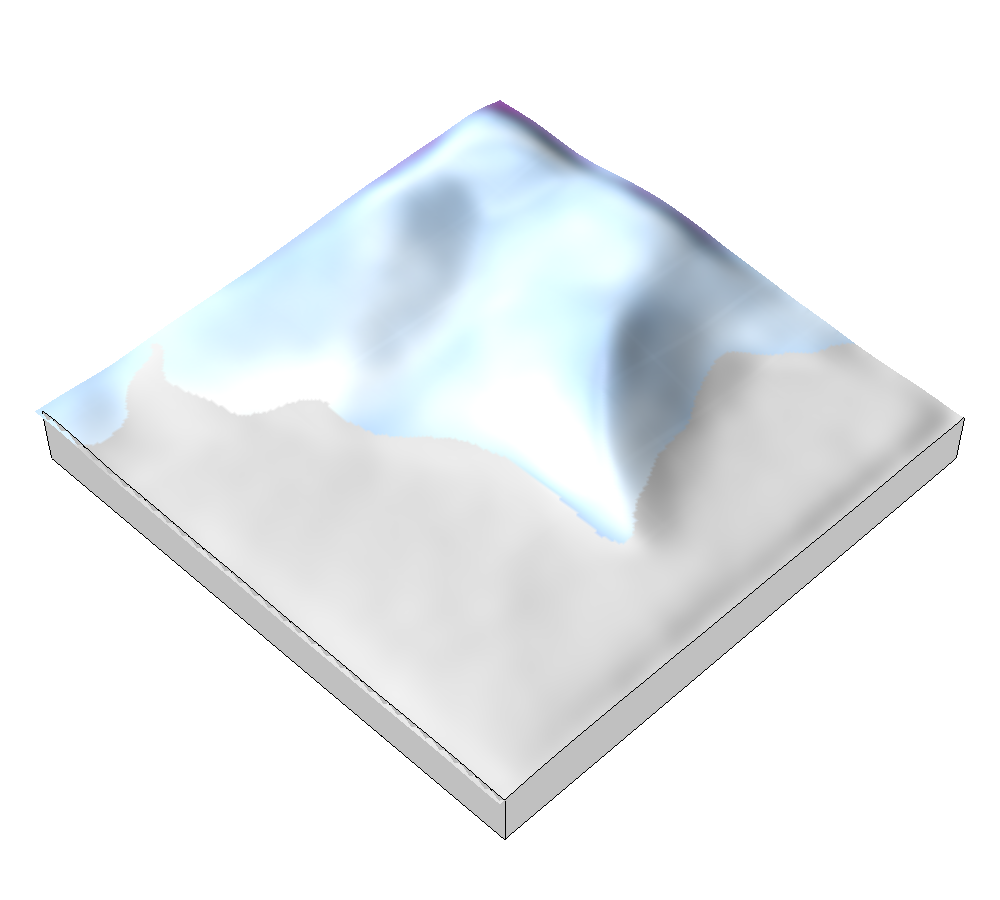
\includegraphics[width=0.18\textwidth]{images/render_3d/participants/stdev_regression_difference_series_3.png}\\
%
Mean difference \par \vspace{0.5em} 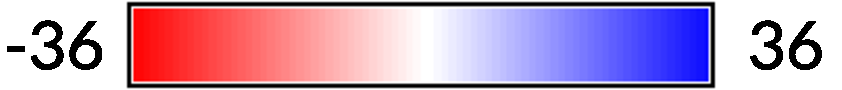
\includegraphics[width=0.16\textwidth]{images/legends/diff_legend.pdf} & 
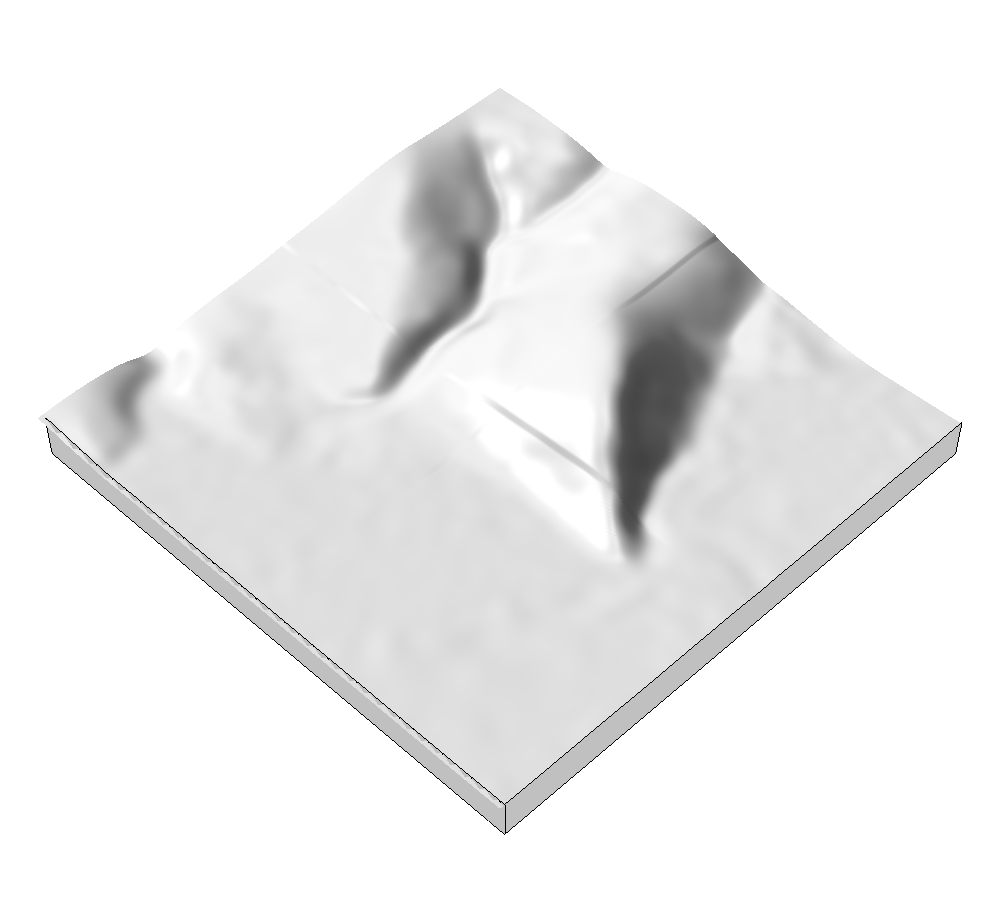
\includegraphics[width=0.18\textwidth]{images/render_3d/participants/dem_difference_1.png} &
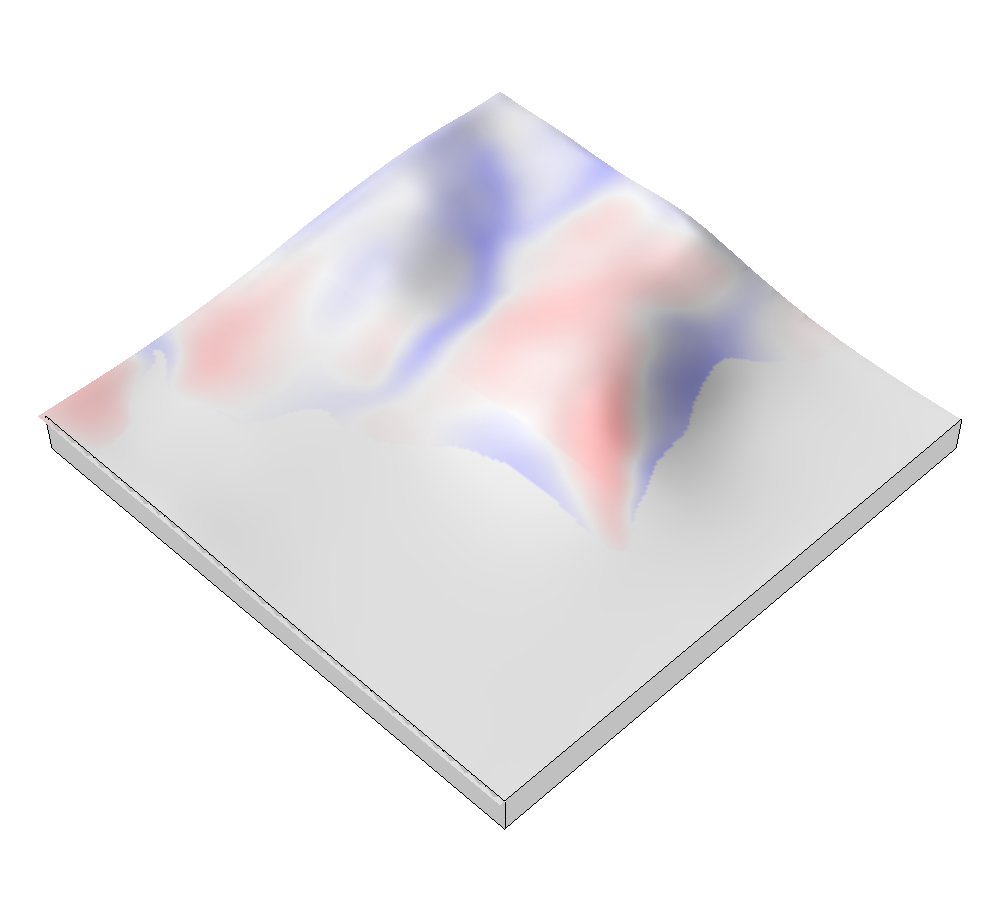
\includegraphics[width=0.18\textwidth]{images/render_3d/participants/mean_dem_regression_difference_1.png} &
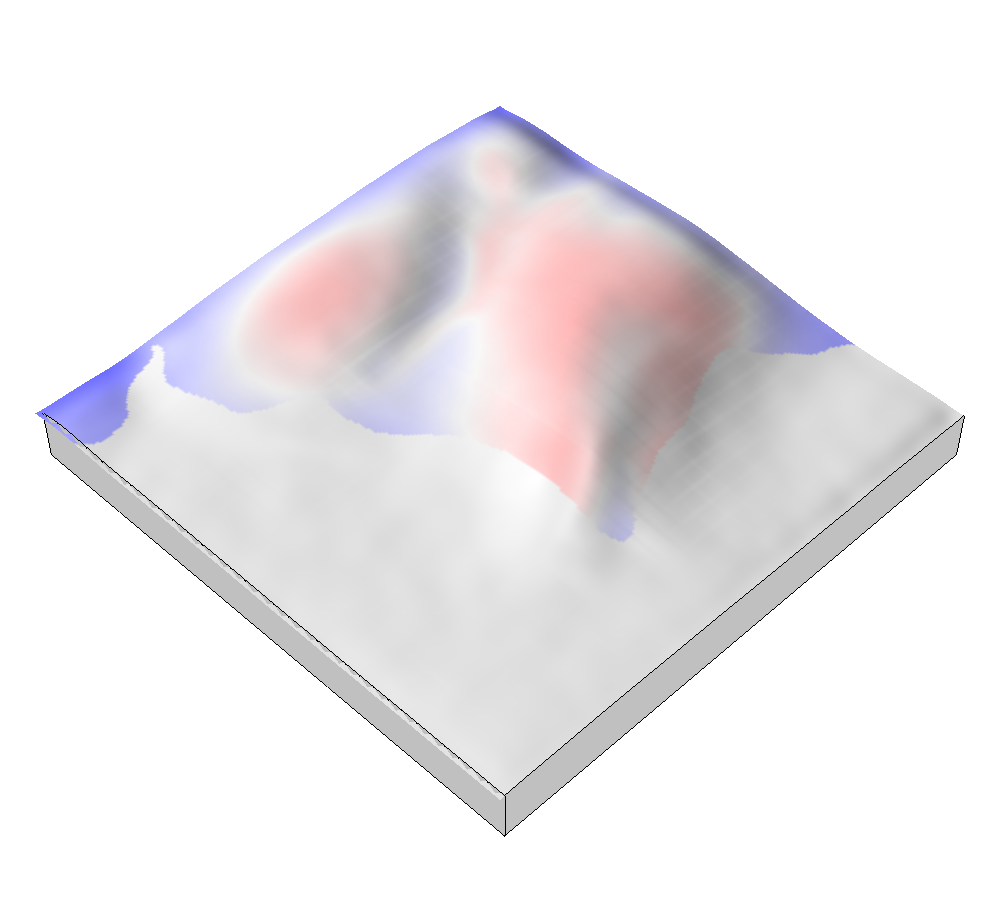
\includegraphics[width=0.18\textwidth]{images/render_3d/participants/mean_dem_regression_difference_2.png} &
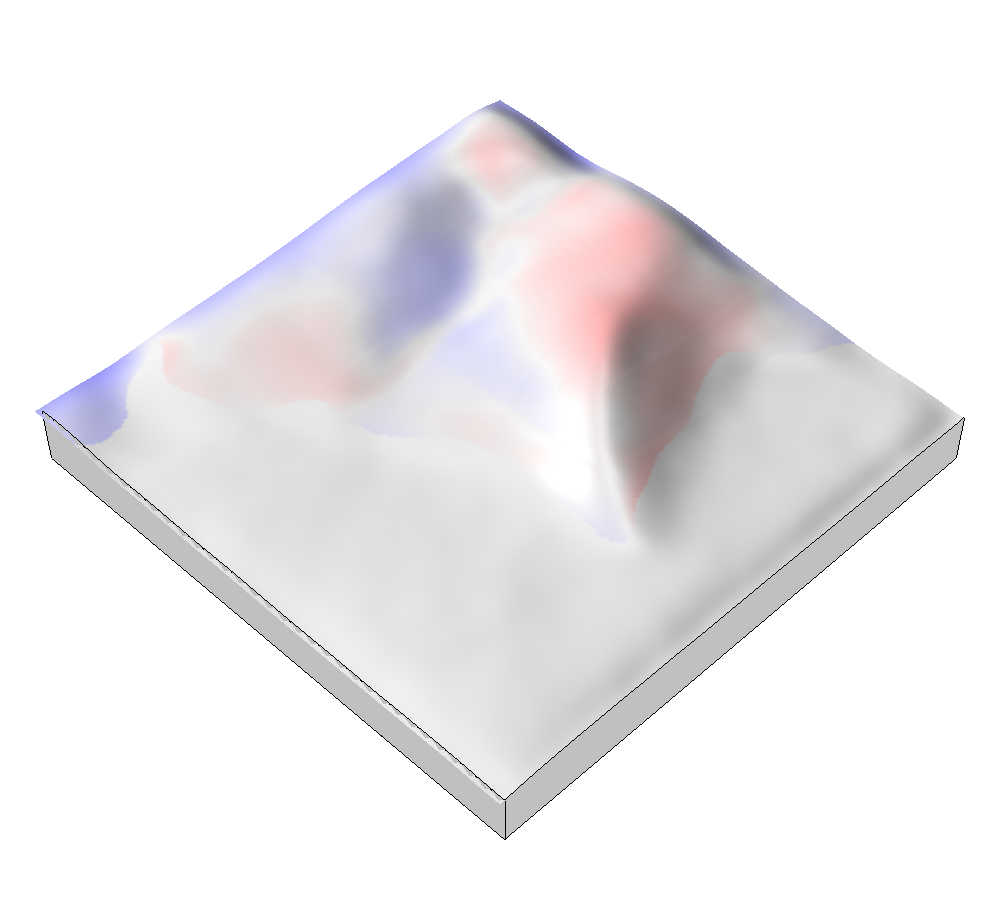
\includegraphics[width=0.18\textwidth]{images/render_3d/participants/mean_dem_regression_difference_3.png}\\
%
Mean slope \par \vspace{0.5em} 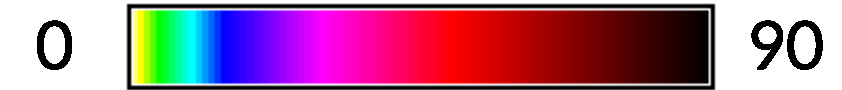
\includegraphics[width=0.16\textwidth]{images/legends/slope_legend.pdf} & 
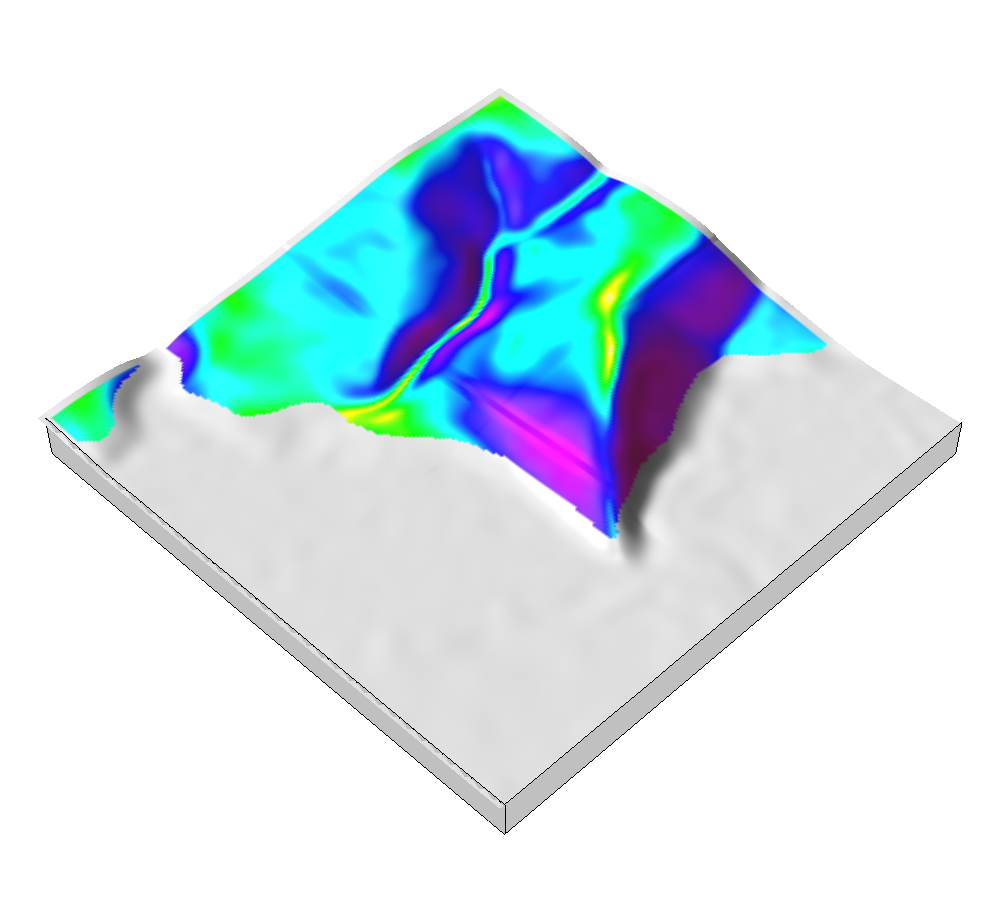
\includegraphics[width=0.18\textwidth]{images/render_3d/participants/slope_1.png} &
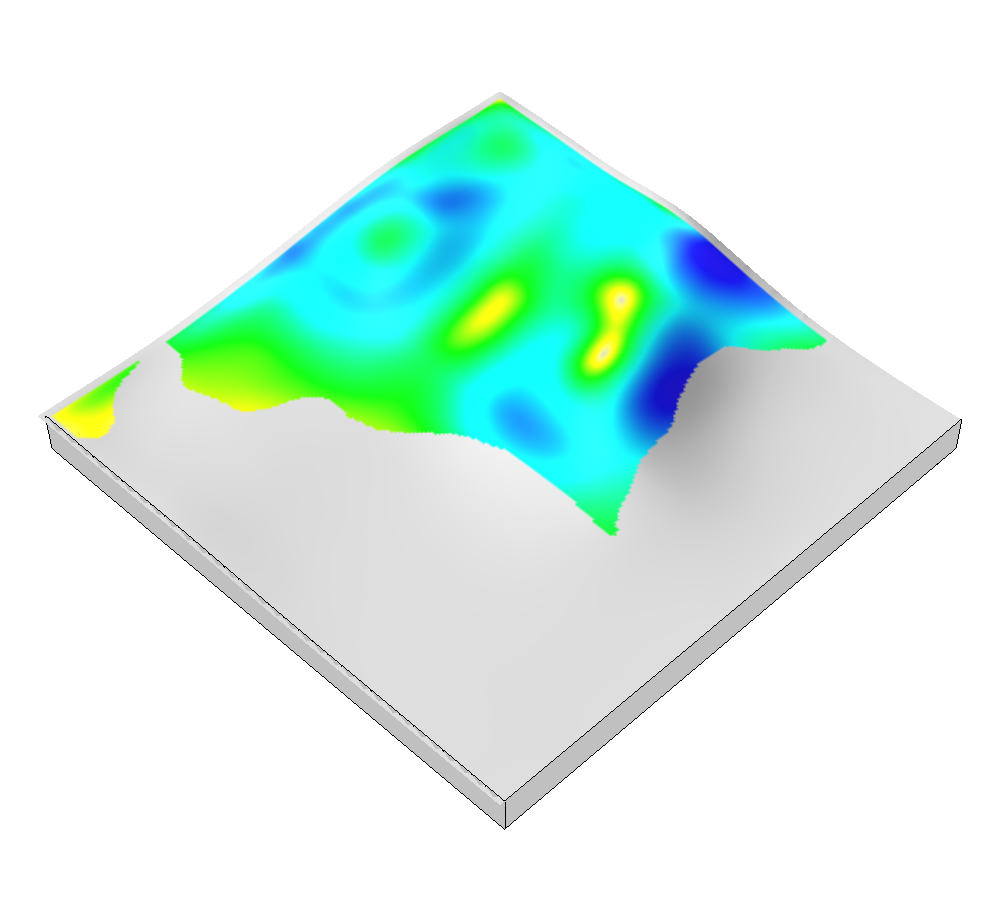
\includegraphics[width=0.18\textwidth]{images/render_3d/participants/mean_slope_1.png} &
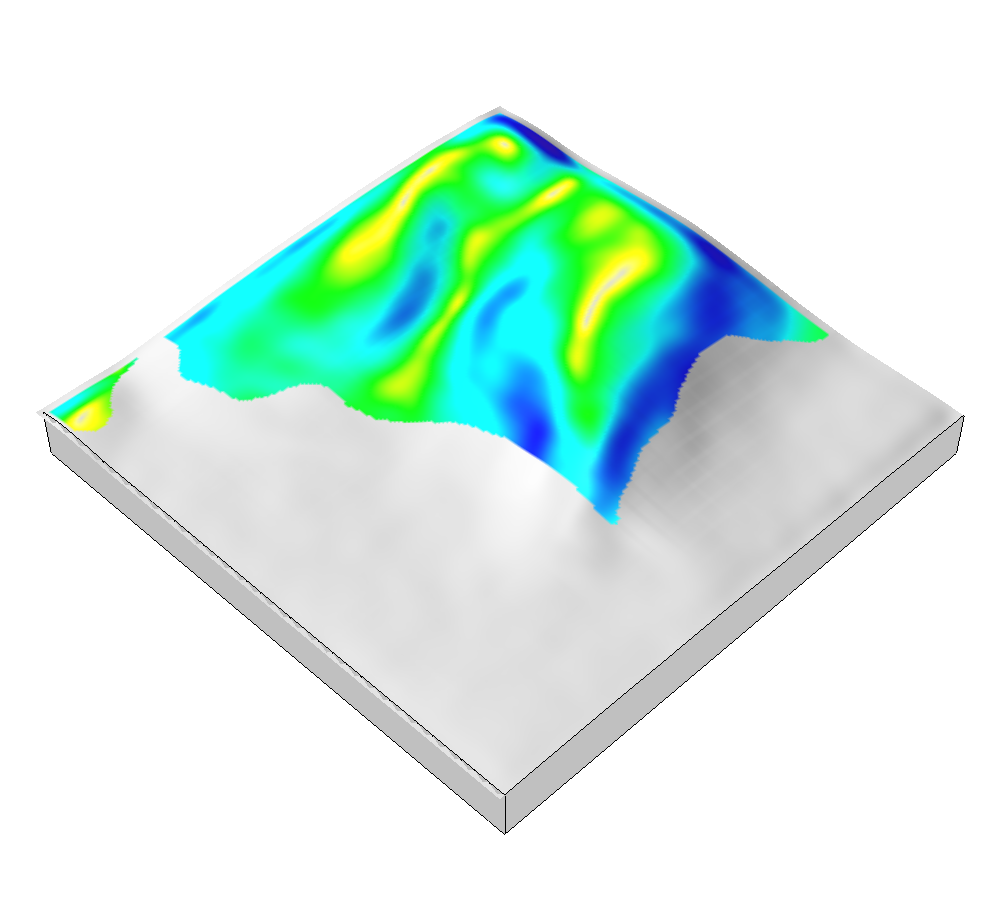
\includegraphics[width=0.18\textwidth]{images/render_3d/participants/mean_slope_2.png} &
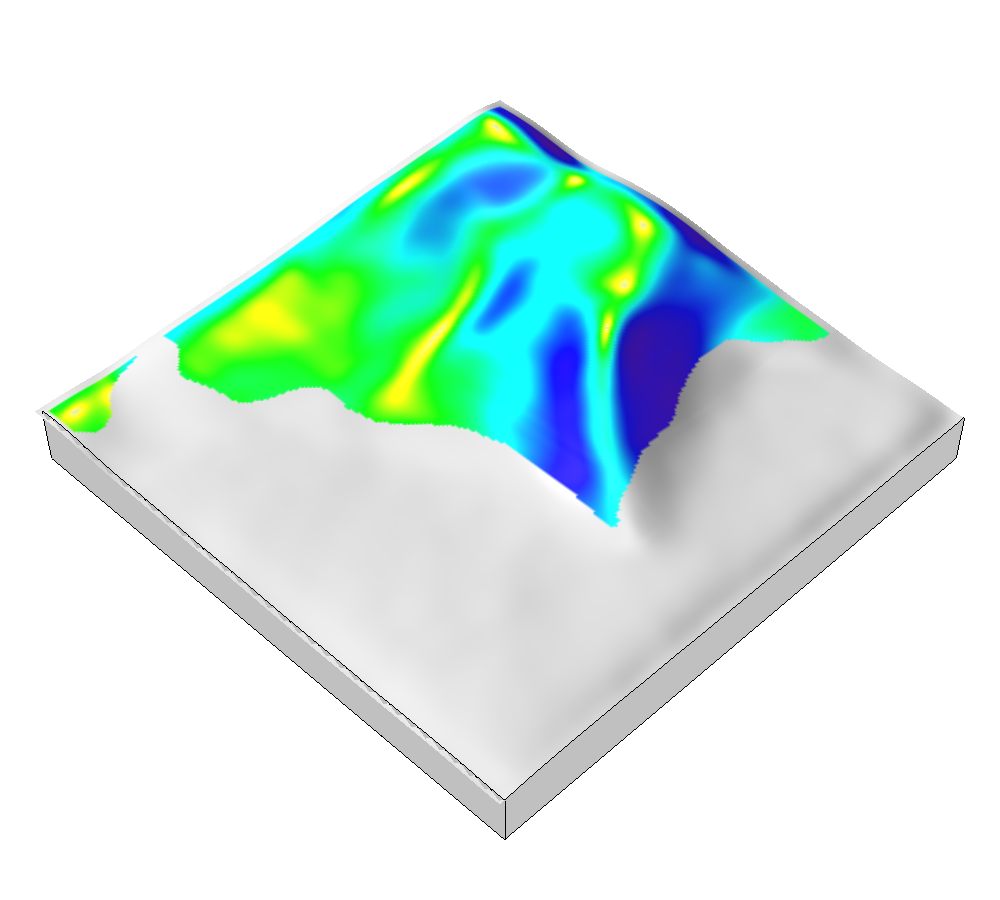
\includegraphics[width=0.18\textwidth]{images/render_3d/participants/mean_slope_3.png}\\
%
Mean landforms \par \vspace{0.5em} 
\includegraphics[width=0.16\textwidth]{images/legends/forms_legend.pdf} & 
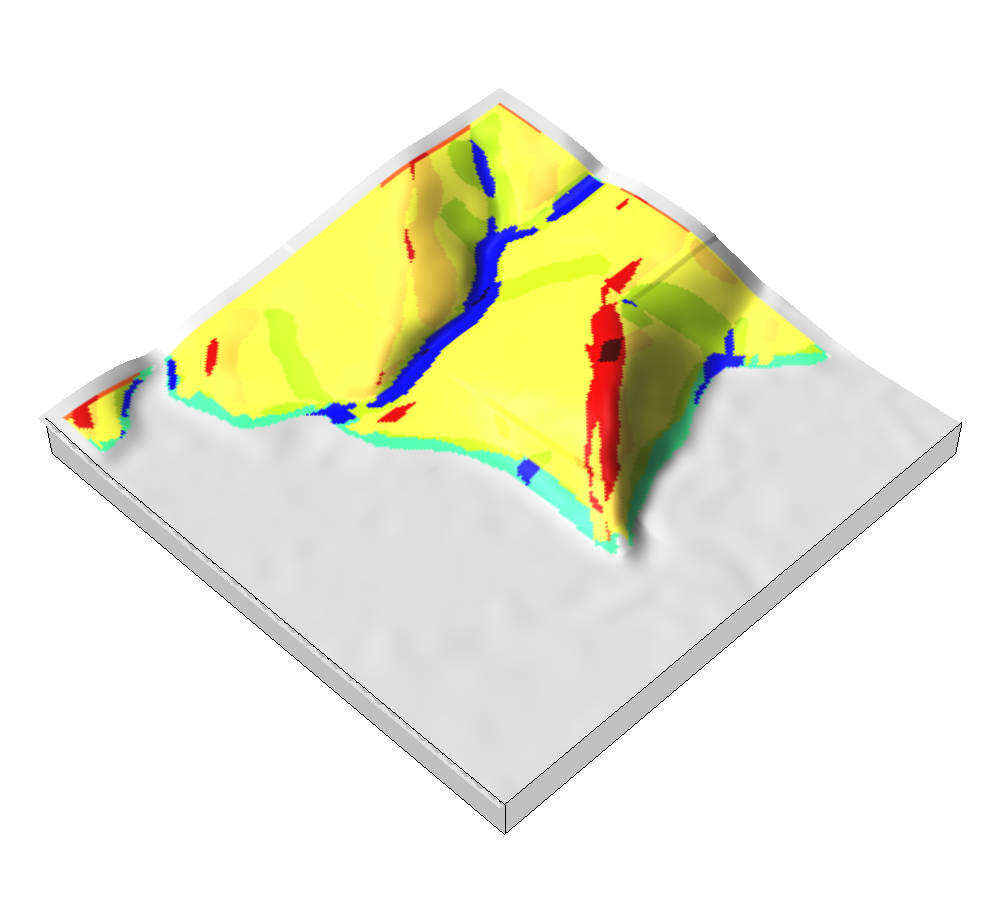
\includegraphics[width=0.18\textwidth]{images/render_3d/participants/forms_1.png} &
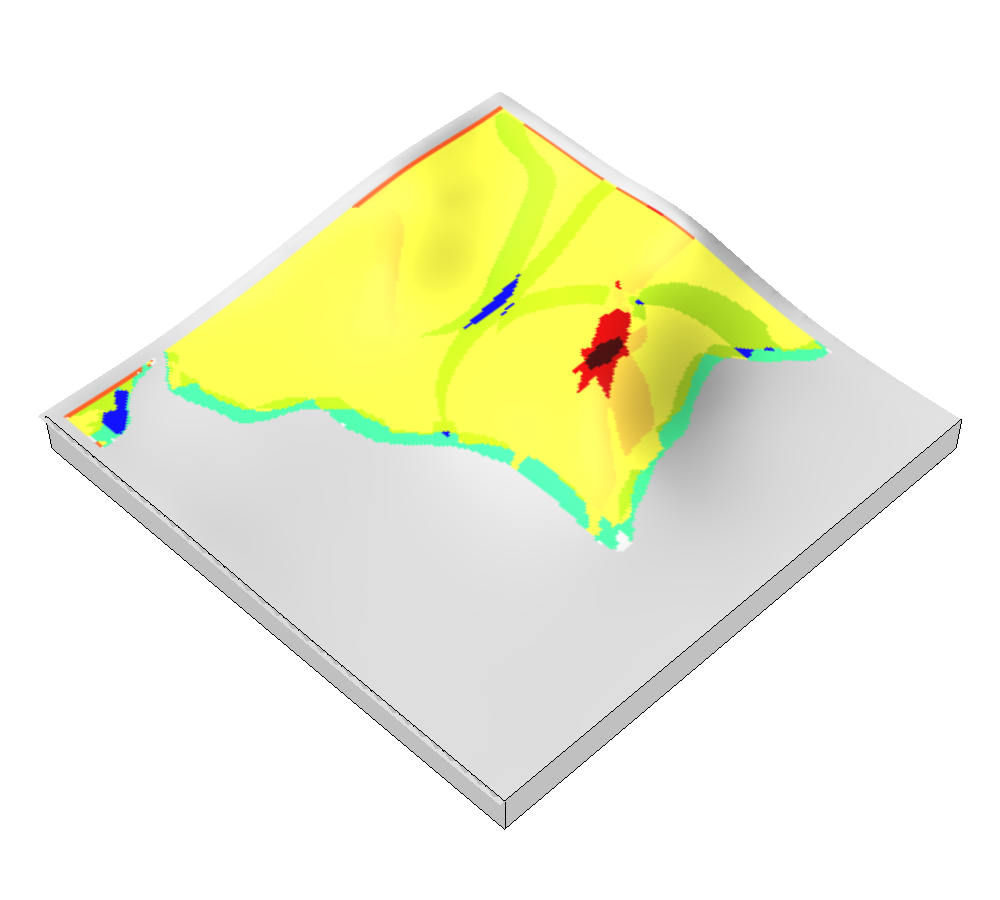
\includegraphics[width=0.18\textwidth]{images/render_3d/participants/mean_forms_1.png} &
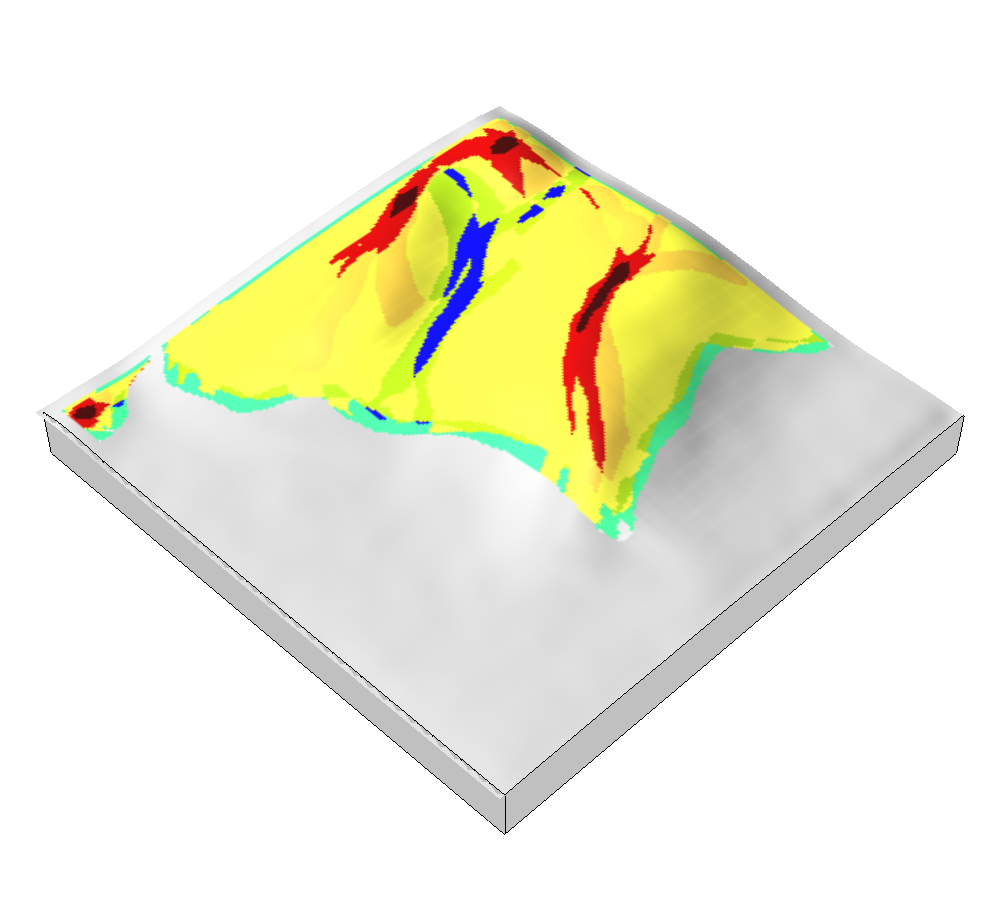
\includegraphics[width=0.18\textwidth]{images/render_3d/participants/mean_forms_2.png} &
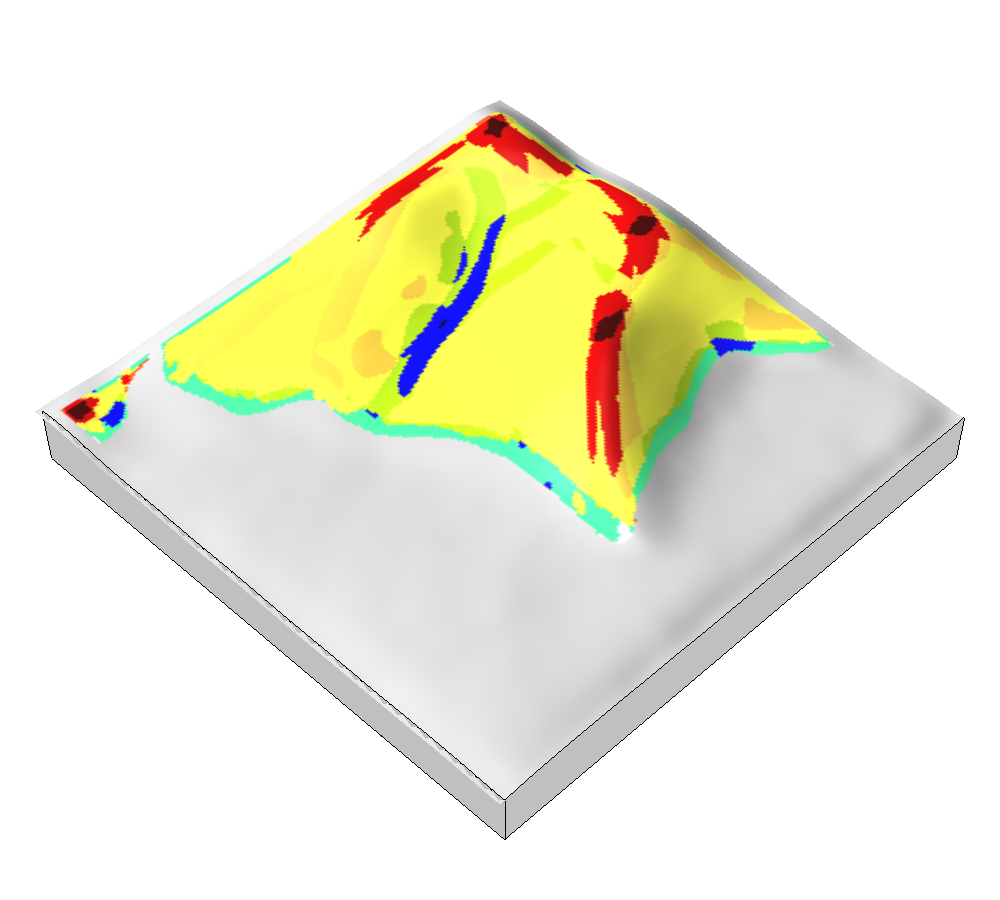
\includegraphics[width=0.18\textwidth]{images/render_3d/participants/mean_forms_3.png}\\
%
\bottomrule
\end{tabular}
\label{table:topography}
%
\vspace*{1.5em}
%
\caption{Landforms identified by \textit{r.geomorphon} in Table~\ref{table:topography}:
		1)~flat, 
		2)~peak, 
		3)~ridge, 
		4)~shoulder, 
		5)~spur, 
		6)~slope, 
		7)~hollow, 
		8)~footslope, 
		9)~valley, and
		10)~depression.
		Source: \cite{r.geomorphon,Jasiewicz2013}}
\vspace*{1em}
\ra{1.3}
\begin{tabular}{m{0.6\textwidth}}
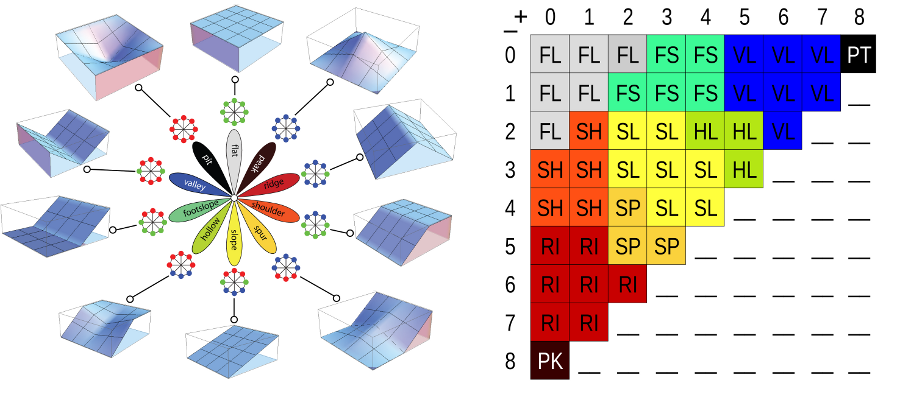
\includegraphics[width=0.6\textwidth]{images/geomorphons_legend.png}\\
\end{tabular}
\label{fig:geomorphons}
%
\end{table*}
